\section{Additional Results}

\begin{figure}[h]
    \centering
    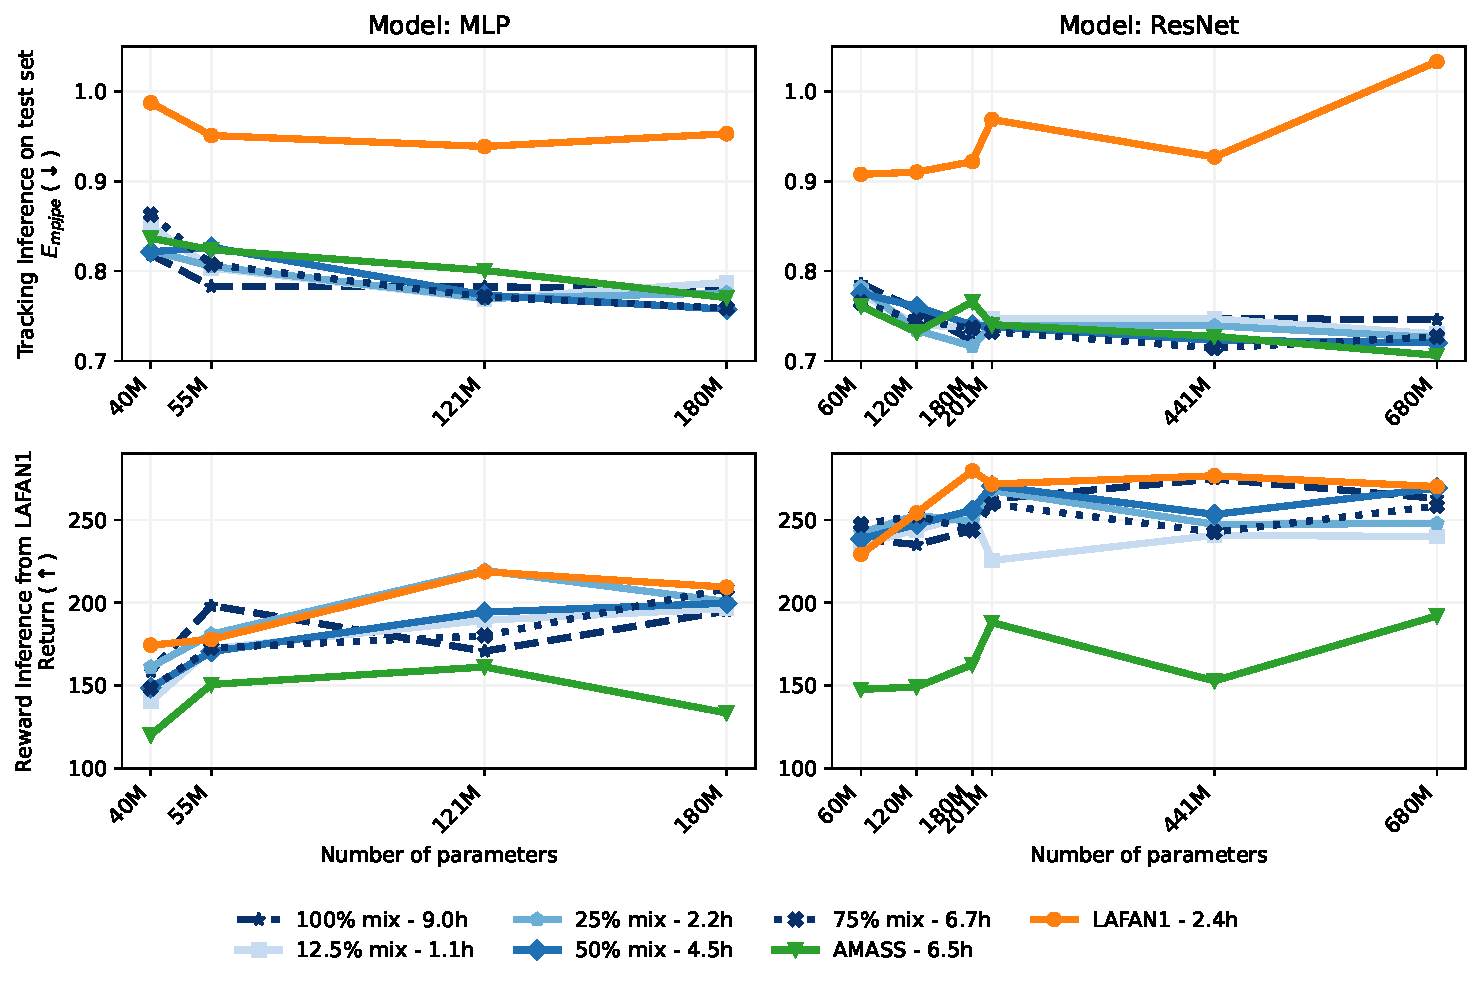
\includegraphics[width=0.96\linewidth]{image/scaling_plot_mix_linear.pdf}
    \caption{Tracking and reward performance on the test set for different models and datasets. The lower the better for tracking and the higher the better for reward.}
    \label{fig:scale_ablation}
\end{figure}

\subsection{Data Size and Model Size}
We perform ablations on both the data and model size. For training the model in the main paper, we used only the LAFAN1 dataset~\citep{HarveyYNP20lafan1}. In these ablations, we additionally leverage motions from the CMU and BMLHandball subsets of AMASS~\citep{Mahmood2019AMASS}. We consider the individual datasets (referred to as LAFAN1 and AMASS in the figure), as well as datasets obtained by merging $X$ percent of the two datasets (with $X = \{12.5\%,25\%,50\%, 75\%, 100\%\}$). We evaluate different network architectures, including simple feed-forward networks and residual architectures with a varying number of blocks (see Tab.~\ref{tab:config}). For tracking, we use the same test dataset as in~\citep{TirinzoniTFGKXL25zeroshot}, but we removed motions from CMU and BMLHandball to ensure complete separation from the training datasets. For reward inference, we use 600,000 samples from the LAFAN1 dataset for all configurations. We report the results of our ablation in Fig.~\ref{fig:scale_ablation} over a single seed.
\begin{table}[h]
\centering
\footnotesize
\begin{tabular}{|cc||cccccc|c|}
\hline
&& \multicolumn{7}{c|}{Number of Parameters}\\
\hline
Architecture & Model & $\pi$ & $Q_R$ & $B$ & $Q_D$ & D & F & Total\\
\hline
ResNet&3-block, 2048dim &19.3M&59.2M&201k&59.2M&2.9M&60.3M&201.1M\\
ResNet$^\star$&6-block, 2048dim &31.9M&134.8M&201k&134.8M&2.9M&135.9M&440.5M\\
ResNet&9-block, 2048dim &44.5M&210.4M&201k&210.4M&2.9M&211.5M&679.9M\\
ResNet&3-block, 1024dim &5.5M&17.0M&201k&17.0M&2.9M&17.6M&60.2M\\
ResNet&6-block, 1024dim &8.6M&36.0M&201k&36.0M&2.9M&36.5M&120.1M\\
ResNet&9-block, 1024dim &11.8M&54.9M&201k&54.9M&2.9M&55.4M&180.1M\\
\hline
MLP&2-layer, 1024dim &4.4M&10.7M&201k&10.7M&2.9M&11.2M&40.1M\\
MLP&2-layer, 2048dim &15.1M&34.0M&201k&34.0M&2.9M&35.0M&121.2M\\
MLP&4-layer, 1024dim &6.5M&14.9M&201k&14.9M&2.9M&15.4M&54.8M\\
MLP&4-layer, 2048dim &23.5M&50.8M&201k&50.8M&2.9M&51.8M&179.9M\\
\hline
\end{tabular}
\caption{Configurations of the architectures and total number of parameters. $\star$ denotes the configuration used in the main paper.}
\label{tab:config}
\end{table}

As we increase the total capacity of the model, tracking performance improves for almost all of the training mocap datasets. LAFAN1 is the only case where performance saturates quite early. We believe this is because the training dataset is a subset of the AMASS dataset, and despite being separated from the training data, it is likely much closer to the motions in CMU and BMLHandball than to those in LAFAN1. We can further notice that residual architectures achieve better performance w.r.t. simple MLP architectures, and we can scale residual architectures to larger sizes. Furthermore, we found training to be instable when scaling MLP to larger architectures.

% \begin{figure}[h]
%     \centering
%     \includegraphics[width=0.96\linewidth]{image/scaling_plot.png}
%     \caption{Tracking and reward performance on the test set for different models and datasets. The lower the better for tracking and the higher the better for reward. We use a log scale for the number of parameters and for the tracking score.}
%     \label{fig:scale_ablation}
% \end{figure}


Similarly, we observe a mild improvement trend for reward inference when increasing the model size. However, training with LAFAN1 (in some proportion) appears to be important in this case, as reward performance drops when we train only with the subset of AMASS. We also evaluated reward inference performance using both the training buffer and the training motion set. In both cases, the average performance decreases, with a much more significant drop when using the training buffer. We believe this may be due to the fact that samples in the buffer are collected with domain randomization, whereas the motion buffers are not randomized. Selecting the optimal dataset for reward inference could be an interesting direction for future research.

% \begin{figure}[h]
%     \centering
%     \includegraphics[width=0.96\linewidth]{image/scaling_plot_rewards.png}
%     \caption{}
%     \label{fig:scale_ablation_rewards}
% \end{figure}

\begin{figure}[h]
    \centering
    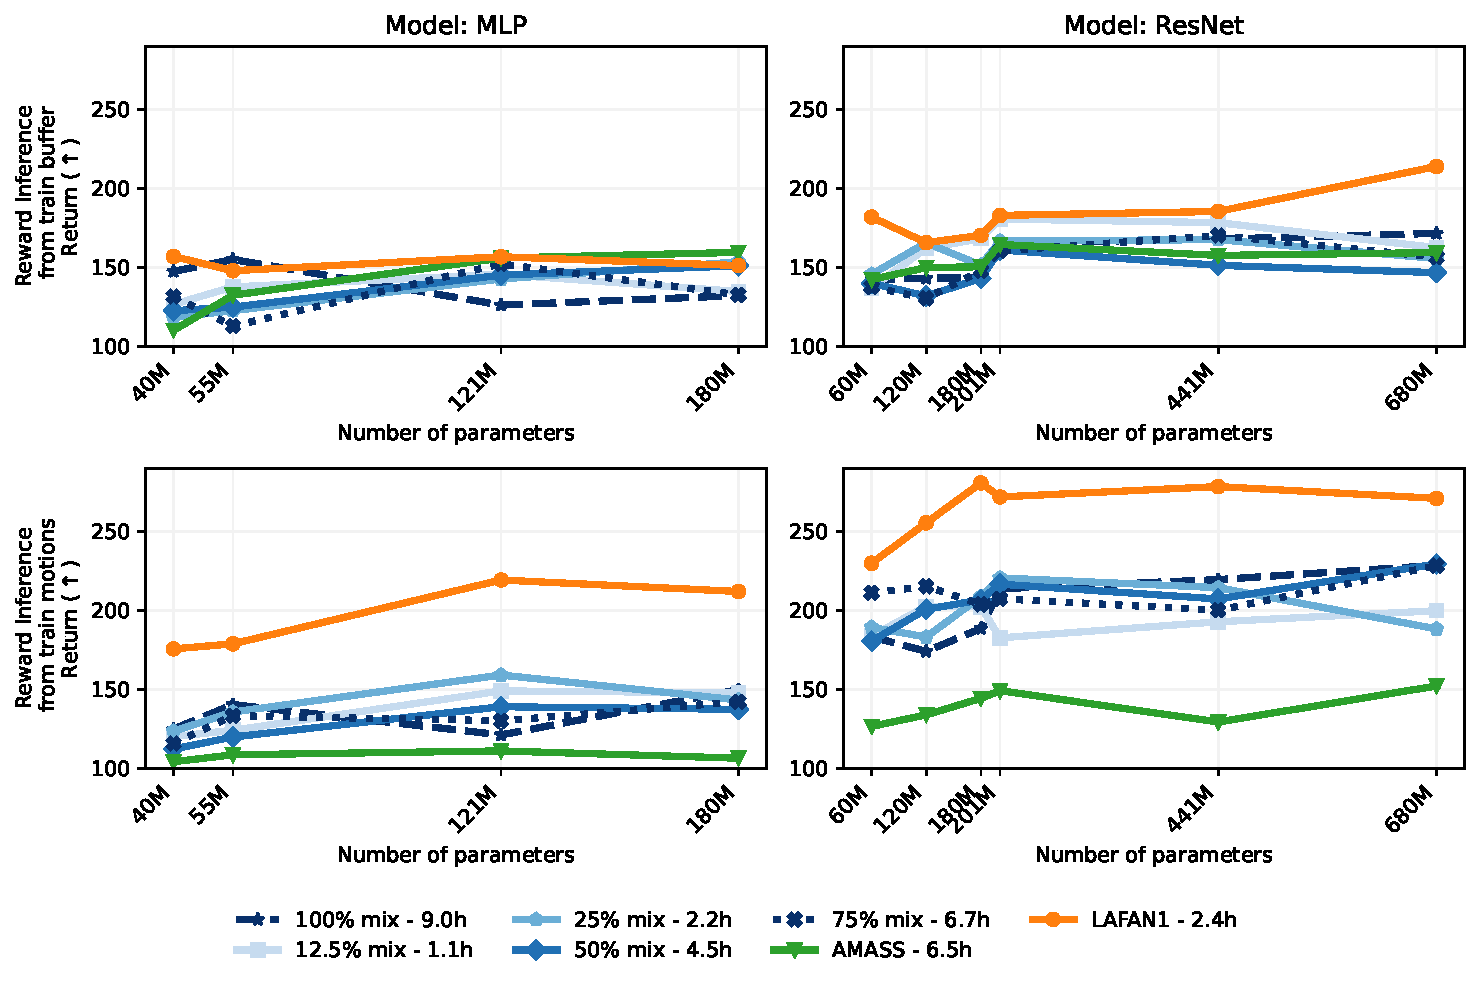
\includegraphics[width=0.96\linewidth]{image/scaling_plot_mix_reward_linear.pdf}
    \caption{Reward inference performance when using the experience generated by the agent (i.e., online replay buffer) or the motion dataset used for training. We get better reward performance when using the motion dataset, in particular when using LAFAN1 (see Fig.~\ref{fig:scale_ablation}).}
    \label{fig:scale_ablation_rewards}
\end{figure}

% \clearpage
\subsection{Application of \method{} on Booster T1}
\label{sec:t1-sim}
We additionally evaluate the generality of our framework by testing \method{} on Booster T1 humanoid robot. The LAFAN1 dataset is retargeted to T1 using LocoMujoco~\citep{alhafez2023b} and we train the policy with exact same hyper-parameters as G1. The algorithm shows strong generalization ability, allowing T1 also to perform natural walking and expressive dancing motions, as shown in~\Cref{fig:t1-sim}.
\begin{figure}[t]
    \centering
    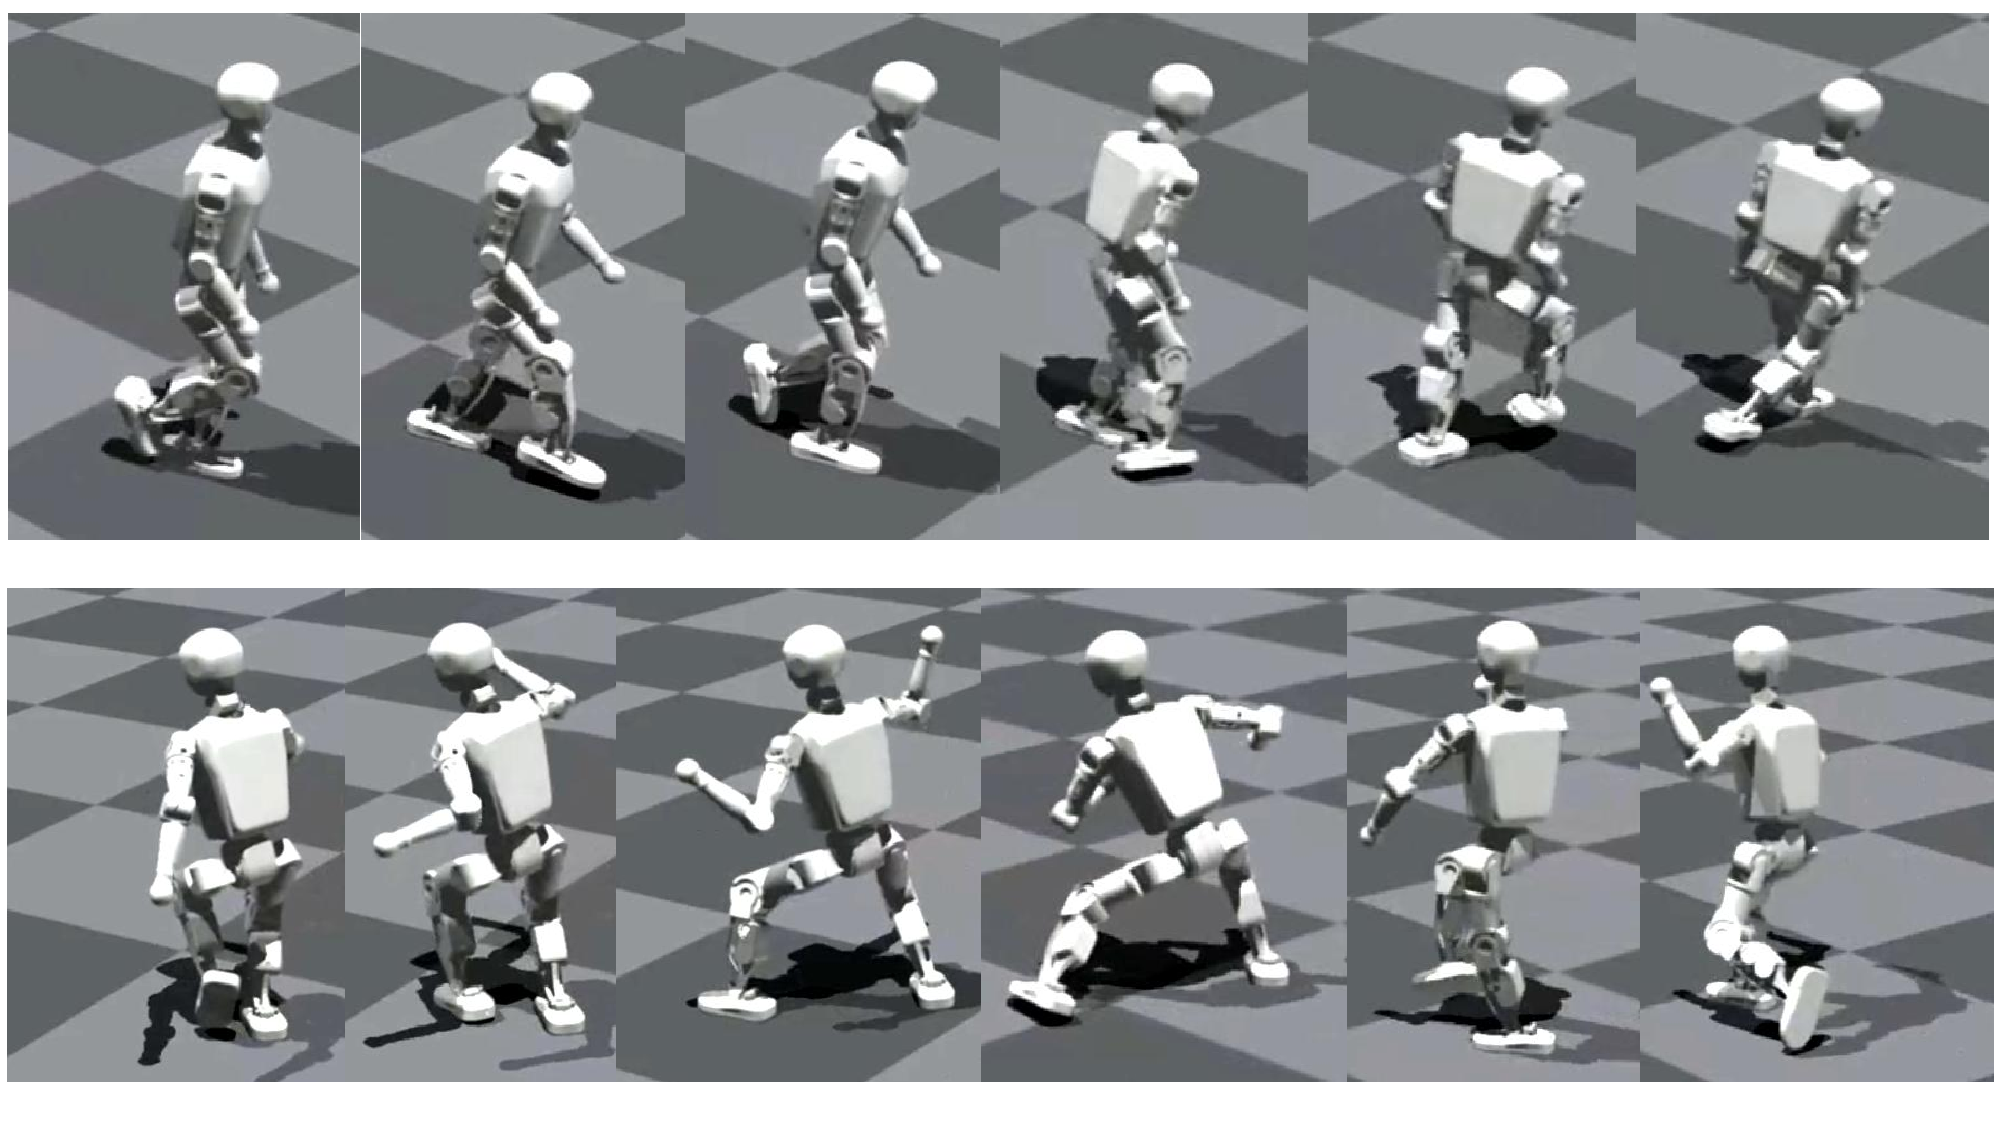
\includegraphics[width=0.7\linewidth]{image/t1_sim.pdf}
    \caption{Application of \method{} on Booster T1.}
    \label{fig:t1-sim}
\end{figure}


% \section{Use of Large Language Models}
% The authors use LLM tools for refining the expression in the final draft of the paper, but did not use it for idea generation, training, and other experiments.